\newpage
\begin{center}
  \textbf{\large 3. Построение преобразователей угол-код на синусно-косинусных решающих устройствах}
\end{center}
\refstepcounter{chapter}
\addcontentsline{toc}{chapter}{3. Построение преобразователей угол-код на синусно-косинусных решающих устройствах}


\section{Классические схемы и их эволюция}

Существует широкий класс схем посмотроения преобразоваталей угол-код.
В литературе, \cite{Vulvet}, описаны различные методы построения преобразователей угол-код. 

\begin{itemize}
  \item Контактные кодирующие преобразователи 
  \item Магниторезистивные преобразователи
  \item Аналоговые схемы с использованием \textbf{RLC-цепей} для формирования сигналов.
  \item Трансформаторные системы, основанные на взаимной индукции.
\end{itemize}

Однако такие решения обладают некоторыми существенными недостатками в современных условиях:
\begin{itemize}
  \item \textbf{Считывание}: Использование моточных изделий (трансформаторов, катушек) увеличивает массу и габариты устройств.
  \item \textbf{Устаревание}: В связи с совершенствованием схем контроллеров, появляются возможности для более оптимальных.
  \item \textbf{Сложность настройки}: Требуется точная подстройка аналоговых компонентов, что снижает надежность.
  \item \textbf{Низкая совместимость} с цифровыми системами управления.
\end{itemize}

Развитие микропроцессорной техники и миниатюризация контроллеров привели к переходу на компактные и энергоэффективные решения. 
Современные преобразователи исключают громоздкие аналоговые компоненты, заменяя их программируемыми схемами.

\section{Современные подходы}

В контексте оптимизации веса, габаритов и точности рассматриваются два основных типа схем:

\begin{enumerate}
    \item \textbf{Цифровые преобразователи на базе микроконтроллеров}:
    \begin{itemize}
        \item Используют АЦП и алгоритмы цифровой обработки сигналов (ЦОС).
        \item Лишены моточных элементов, что снижает массу на 30–40\%.
        \item Обеспечивают точность до \(\pm0.1^\circ\) за счет программной компенсации погрешностей.
    \end{itemize}
    
    \item \textbf{Гибридные схемы с интегрированными ИС}: 
    \begin{itemize}
        \item Комбинируют аналоговые синусно-косинусные генераторы и цифровые интерфейсы (SPI, I\(^2\)C).
        \item Применяют специализированные микросхемы (например, AD2S1210), минимизирующие число внешних компонентов.
        \item Поддерживают разрешение до 16 бит при компактных размерах.
    \end{itemize}
    Например на рынке доступна микросхема К1310НМ025. \cite{Spec}
\end{enumerate}

\subsection{Преимущества современных решений}
\begin{itemize}
    \item \textbf{Миниатюризация}: Отказ от трансформаторов снижает объем устройства в 2–3 раза.
    \item \textbf{Повышенная надежность}: Цифровая обработка исключает дрейф параметров аналоговых компонентов.
    \item \textbf{Совместимость}: Интеграция с промышленными сетями (CAN, Ethernet) упрощает внедрение.
\end{itemize}

Таким образом, классические схемы, описанные в ранних работах, уступают современным цифровым и гибридным решениям по ключевым параметрам. 
Переход на микроконтроллерные системы и специализированные ИС позволяет достичь высокой точности при минимальных массогабаритных показателях, 
что особенно актуально для аэрокосмических и робототехнических применений

В части цифровой обработки сигналов датчиков рассматриваются две основные схемы:
\begin{itemize}
    \item Метод прямого преобразования
    \item Следящее преобразование
\end{itemize}
Рассмотрим их подробнее.

\subsection{Метод прямого преобразования}
\subsubsection{Принцип работы}
Метод прямого преобразования \cite{Armenski} основан на вычислении угла поворота через арктангенс отношения синусоидального (\(U_{\sin}\)) и косинусоидального (\(U_{\cos}\)) сигналов:
\[
\theta = \arctan\left(\frac{U_{\sin}}{U_{\cos}}\right).
\]
Для реализации метода используются два АЦП, оцифровывающих сигналы с датчика. Разрядность АЦП напрямую влияет на точность: 
\[
\Delta\theta = \frac{360^\circ}{2^N},
\]
где \(N\) — разрядность АЦП. Например, для \(N = 12\) бит:
\[
\Delta\theta = \frac{360^\circ}{4096} \approx 0.088^\circ.
\]

\subsubsection{Проблемы метода}
Метод прямого преобразования угла в код через вычисление арктангенса отношения синусоидального и косинусоидального сигналов сталкивается со следующими ограничениями:
\begin{itemize}
    \item \textbf{Зависимость от качества сигналов} \\
    Шумы, нелинейности и фазовые сдвиги в сигналах \( U_{\sin} \) и \( U_{\cos} \) приводят к систематическим ошибкам. Например, асимметрия амплитуд вызывает погрешность:
    \[
    \Delta\theta = \arctan\left(\frac{U_{\sin} + \delta}{U_{\cos}}\right) - \arctan\left(\frac{U_{\sin}}{U_{\cos}}\right),
    \]
    где \(\delta\) — отклонение амплитуды.

    \item \textbf{Высокие требования к АЦП} \\
    Для точности \(\Delta\theta < 0.1^\circ\) требуется разрядность АЦП не менее 16 бит:
    \[
    N = \log_2\left(\frac{360^\circ}{\Delta\theta}\right) \approx 16.
    \]

    \item \textbf{Нелинейности и калибровка} \\
    Отклонения от идеальной синусоиды требуют использования таблиц поправок, увеличивая сложность алгоритма. Появляющеся в процессе работы нелинейности скомпенсированы не будут.

    \item \textbf{Чувствительность к внешним факторам} \\
    Температурный дрейф компонентов (например, АЦП) снижает стабильность:
    \[
    \Delta\theta_{\text{дрейф}} = \alpha \cdot \Delta T,
    \]
    где \(\alpha\) — температурный коэффициент, \(\Delta T\) — перепад температуры.

    \item \textbf{Проблемы при малых сигналах} \\
    При \(\theta \to 0^\circ\) или \(90^\circ\) отношение \( U_{\sin}/U_{\cos} \) стремится к \(0\) или \(\infty\), увеличивая погрешность из-за дискретизации.
\end{itemize}

Таким образом метод прямого преобразования подходит для статических систем с умеренными требованиями к точности. 
В динамических или высокоточных приложениях предпочтительны преобразователи с обратной связью, компенсирующие перечисленные недостатки.

\subsection{Следящие преобразователи}
\subsubsection*{Принцип работы}
Следящие преобразователи (СП) используют замкнутый контур управления для минимизации рассогласования между текущим углом и заданным значением. 
Сигналы \(U_{\sin}\) и \(U_{\cos}\) сравниваются с опорными, а ошибка подается на корректирующий элемент (например, двигатель). \cite{Anufriev2014} \cite{Safronov}

\subsubsection{Структура СП}
\begin{itemize}
    \item \textbf{Фазовый детектор}: Вычисляет разность фаз между входными и опорными сигналами.
    \item \textbf{Интегратор}: Формирует управляющий сигнал для исполнительного механизма.
    \item \textbf{Обратная связь}: Обеспечивает точность \(\pm0.01^\circ\) за счет коррекции в реальном времени.
\end{itemize}

\subsubsection{Современные подходы к реализации}
Следящие преобразователи обеспечивают прецизионное управление в динамических системах, но требуют сложной настройки.
Поэтому чаще всего для обсчета используются программируемые логические интергальные схемы (ПЛИС) или микроконтроллеры.\cite{MilandrSKVT}

\section{Техническое задание на устройство}
Разрабатываемая система состоит двух датчиков СКВТ и применение специализированной микросхемы потребовало бы использование двух ИС, по одной на каждый датчик.
В связи с дороговизной этих устройств и возмодных проблемах с поставкой, было принято решение о собственной разработке печатного узла на основе микроконтроллера stm32 с ядром F7.
По мтога проведенных научно-исследовательских мероприятий было составлено техническое задание на устройство с целью обеспечить требуемые характеристики.

\subsection{Назначение и состав изделия}
Требуемый печатный узел представляет из себя блок аналого-цифрового преобразователя вращающегося трансформатора (АЦПВТ) предназначен для определения углового положения 
одной из координат антенной системы. 
Работа АЦПВТ ведется по двухотсчетной схеме с величиной редукции от датчика грубого отсчета к датчику точного отсчета 1/36.  

\subsection{Основные технические требования}
\begin{itemize}
    \item На рисунке ~\ref{FuncBlocks}, упрощенно показана структурная схема изделия. 
          С помощью разъема СНП-59 блок подключается к датчикам углового положения и концевым выключателям приборного редуктора. 
          Внутри блока расположены схемы обработки сигналов вращающихся трансформаторов и концевых выключателей. 
          Преобразованные с помощью данных схем сигналы затем отправляются ведущему устройству с помощью микроконтроллера и приемо-передатчика.  

    \item Дополнительно в изделии установлен разъем, подключенный параллельно концевым выключателям приборного редуктора с целью реализации цепей безопасности: 
          подключение невозвратных концевых выключателей последовательно в цепь питания главного контактора шкафа электропривода. 

        \begin{figure}[!t]
          \centering
          \includegraphics[width=150mm ]{FuncBlocks.jpg} 
          \caption{Эскиз функциональных блоков изделия}
          \label{FuncBlocks}
        \end{figure}

    \item Изделие должно функционировать с вращающимися трансформаторами типа ЛИР-ДР158А.
      \end{itemize}


    В качестве интерфейса информационного обмена должен использоваться последовательный SSI со следующими параметрами:
    \begin{itemize}
          \item Частота следования импульсов сигнала «Clock» 100кГц,
          \item Формирование телеграммы блока АЦПВТ должно происходить с использованием кода Грея. 
          \item В телеграмме 18 бит, начиная со старшего (MSB), должны быть использованы для передачи углового положения координаты антенны. 
    \end{itemize}

\subsection{Конструктивные требования}

    Конструктивно блок АЦПВТ должен представлять из себя картридж, который вставляется в корпус приборного редуктора. 
    После стыковки блока АЦПВТ и приборного редуктора обеспечивается герметичность узла. 

    Cхема блока размещена на одной печатной плате, габариты которой задаются эскизом корпуса блока АЦПВТ (см. рисунки \ref{Corp1}, \ref{Corp2}). 

    \begin{figure}[!t]
      \centering
      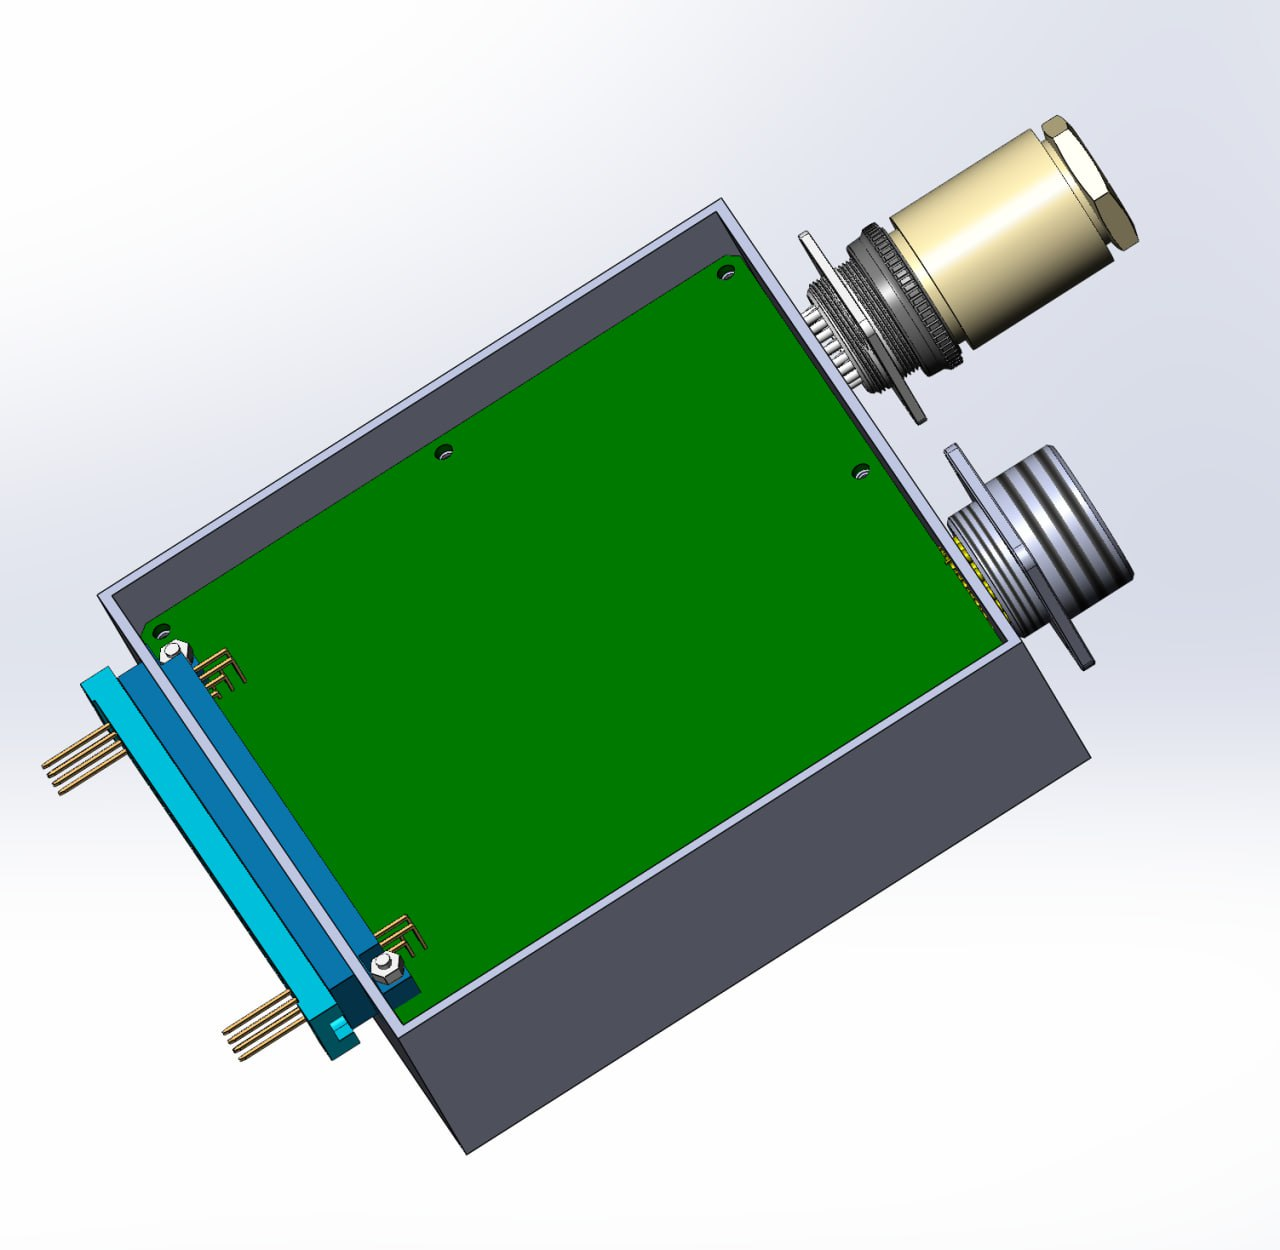
\includegraphics[width=150mm ]{Corp1.jpg} 
      \caption{Корпус блока}
      \label{Corp1}
    \end{figure}

    \begin{figure}[!t]
      \centering
      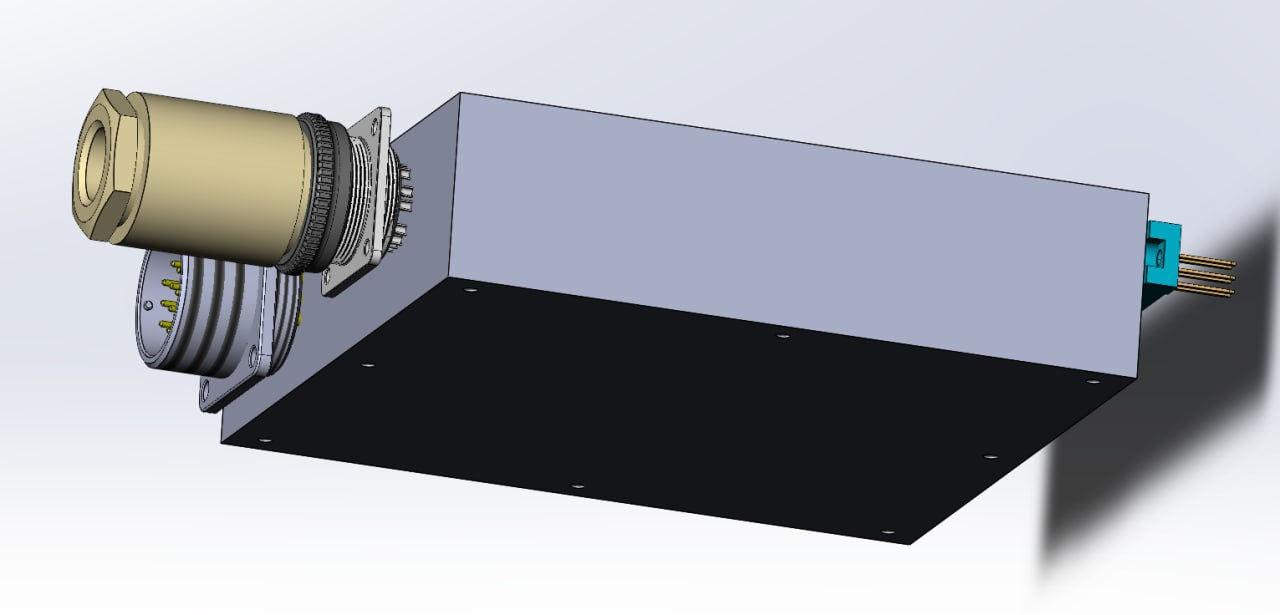
\includegraphics[width=150mm ]{Corp2.jpg} 
      \caption{Корпус блока}
      \label{Corp2}
    \end{figure}

\subsection{Требования по устойчивости к внешним воздействиям}
  К печатному узлу предъявляются жесткие требования по стойкости к воздействию климатических факторов:
\begin{itemize}

  \item пониженная температура рабочая – минус 40°С;

  \item пониженная температура предельная – минус 60°С;

 \item повышенная температура рабочая – плюс 60°С;

 \item повышенная температура предельная – плюс 70°С;

 \item относительная влажность – до 95 процентов при температуре плюс 30°С;

 \item иней и роса – температура минус 25°С, длительность воздействия до 2 часов;
 
\end{itemize}


\section{Узел печатный}

По итогу проведёной разработки, был изготовлен узел печатный блока АЦПВТ. Для создания возбуждающего синусоидального сигнала был выбран внешний ЦАП, сигнал с которого "раскачивается" с (0-3.3)В,
до требуемых датчику ЛИР-ДР158А для возбуждения (-7 - 7)В, с помощью схемы с полевыми транзисторами. Цифровой параллельный вход ЦАП для удобства функционирования подключен 
к отдельному порту микроконтроллера. 

Для обработки сигналов двух датчиков установлены две внешние микромхемы АЦП, на каждый их них также выделено по отдельному порту. 

Для аппратной синхронизации подачи управляющих сигналов на внешние микромхемы была реализована схема 
работы аппаратных таймеров в режиме взаимодействия ведущий - ведомый. (см. рис. ~\ref{Timers})

\begin{figure}[!h]
  \centering
  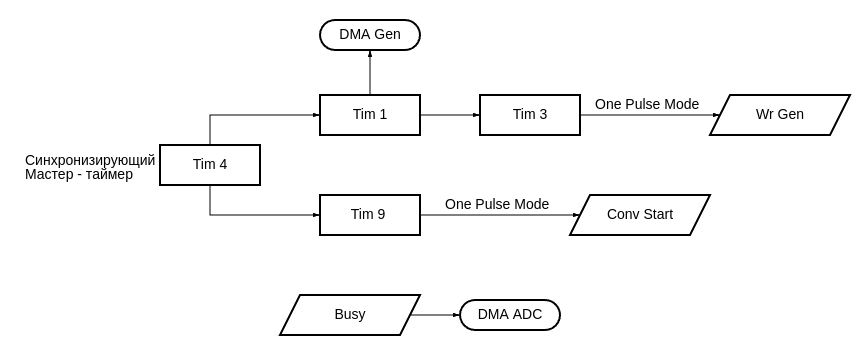
\includegraphics[width=150mm ]{TimersScheme1.png} 
  \caption{Схема взаимодействия таймеров}
  \label{Timers}
\end{figure}

Мастер-таймер 4 синхронно запускает таймеры 3 и 9. Таймер 3 запускает DMA (Direct Memory Access - переферия для доступа в память без участия процессора) на передачу нового значения в порт ЦАП.
После передачи он в режиме one-pulse-mode подает сигнал (Write Gen) на пин микросхемы, начиная загрузку значения из параллельного порта во внутренний регистр ЦАП. Таймер 9 нужен для задержки подачи
сигнала начала преобразования АЦП (Conversion start), чтобы реализовать взятие выборки по амплитуде ответного сигнала с датчика ЛИР-ДР158 и  использовать весь размах напряжения, 
увеличивая тем самым точность расчетов.

Получение данных с параллельного порта АЦП происходит также посредствам DMA в момент получения прерывания по спадающему фронта сигнала Busy. Так как этот сигнал через логические "ИЛИ" 
заведен на все 4 микросхемы АЦП, то значения снимаются со всех АЦП после окончания преобразования последнего. 
\textbf{схемы включения АЦП и ЦАП}

\textbf{Картинка синуса с ЦАП}

Таким образом, путем использования аппаратных моудлей, была достигнута максимальная производительность и временная точность работы микроконтроллера, 
позволяя оставить процессорное время на обработку концевых выключателей и взимодействие с внутренней экосистемой компании по средствам инстерфейса CAN.

\section{Разработка следящего алгоритма}
После отладки аппаратной работы микросхем, встала задача реализации алгороитма расчета углов. 
В рамках разработки системы обработки сигналов датчиков угловых перемещений ЛИР-ДР158А был выбран метод следящего преобразования, так как данный метод,
 позволяет минимизировать систематические ошибки и повысить разрешающую способность преобразователя. 
 Ключевая особенность, критически важная в разраюатываемом устройстве, заключается в использовании контура обратной связи, компенсирующего фазовые и скоростные рассогласования.

\subsection{Реализация следящего алгоритма}
Структурная схема следящего преобразователя представлена на схеме рис. \ref{fig:tracking_scheme}. 

\begin{figure}[ht]
  \resizebox{150mm}{!}{%
  \begin{tikzpicture}[
      block/.style={
          rectangle, 
          draw, 
          text width=6em, 
          text centered, 
          minimum height=3em, 
          font=\small,
          rounded corners=3pt
      },
      arrow/.style={->, thick, >=stealth},
      node distance=1.2cm and 0.8cm,
    ]
  
  % Блоки
  \node[block] (multSin) {Умножитель на $\sin(\phi')$};
  \node[block, below=of multSin] (multCos) {Умножитель на $\cos(\phi')$};
  \node[block, right=of multSin] (detector) {Детектор ошибки};
  \node[block, right=of detector] (integrator) {Интегратор угла};
  
  % Сигналы
  \node[left=of multSin] (inputSin) {$ V sin(\omega t) sin(\phi)$};
  \node[left=of multCos] (inputCos) {$ V sin(\omega t) cos(\phi)$};
  \node[right=of integrator] (output) {$\omega$};
  
  % Обратная связь: phi' к умножителям
  \coordinate (feedback) at ($(integrator.east)!0.5!(output.west)$);
  \node[above=0.3cm of feedback, font=\scriptsize] {};
  \draw[arrow, dashed, red] (integrator.north) -- ++(0.5cm,0) |- ([yshift=1cm]multSin.north) -- (multSin.north);
  \draw[arrow, dashed, red] (integrator.south) -- ++(0.5cm,0) |- (multCos.east); %([yshift=1cm]multCos.south) -- 
  
  % Основные соединения
  \draw[arrow] (inputSin) -- (multSin);
  \draw[arrow] (inputCos) -- (multCos);
  \draw[arrow] (multSin) -- (detector);
  \draw[arrow] (multCos) -- (detector);
  \draw[arrow] (detector) -- node[below=0.7cm] {} (integrator);
  \draw[arrow] (integrator) -- (output);
  
  % Пояснение обратной связи
  \node[above=0.1cm of multSin, align=center, font=\scriptsize] {};
  \node[below=0.1cm of multCos, align=center, font=\scriptsize] {Обратная связь: \\ $\phi'$ обновляется \\ через интегратор};
  
  \end{tikzpicture}
  } % Конец resizebox
  \caption{Схема следящего преобразователя с обратной связью.} % Красные пунктирные линии показывают передачу оценки угла $\phi'$ обратно в умножители.
  \label{fig:tracking_scheme}
  
  \end{figure}
  

Алгоритм включает следующие этапы:
\begin{enumerate}
    \item \textbf{Умножение сигналов:} Входные сигналы \( V_{\text{sin}} \) и \( V_{\text{cos}} \) умножаются на синтезированные опорные сигналы \( \sin(\phi') \) и \( \cos(\phi') \), где \( \phi' \) — текущая оценка угла. 
    \item \textbf{Детектирование ошибки:} Результирующий сигнал ошибки формируется как: 
    \begin{equation}
      e = V sin(\omega t) sin(\phi) \cdot cos(\phi') - V sin(\omega t) cos(\phi) \cdot sin(\phi') = V sin(\omega t) \cdot \sin(\phi - \phi'),
      \label{eq:error}
    \end{equation}
    % \[
    % e = V sin(\omega t) sin(\phi) \cdot cos(\phi') - V sin(\omega t) cos(\phi) \cdot sin(\phi') = V sin(\omega t) \cdot \sin(\phi - \phi') .
    % \]
    Для малых рассогласований \( \phi - \phi' \) ошибка пропорциональна разности углов ($\sin(\phi - \phi') \approx \phi - \phi'$).
    \item \textbf{Интегрирование:} Сигнал ошибки интегрируется для расчёта угловой скорости \( \omega \), а затем — угла \( \phi' \). 
    \begin{equation}
      \phi'(t) = \phi'(0) K_i \int_0^t \sin\left(\phi(\tau) - \phi'(\tau)\right) d\tau, 
      \label{eq:phi_prime}
    \end{equation}
      
      где:
    \begin{itemize}
        \item \(K_i\) — коэффициент усиления интегратора,
        \item \(\phi(\tau)\) — истинный угол (измеряемый датчиком),
        \item \(\phi'(0)\) — начальное условие (оценка угла в момент \(t=0\)).
    \end{itemize}


    %Интегратор устраняет постоянную составляющую ошибки, обеспечивая нулевую погрешность при постоянной скорости вращения.
\end{enumerate}

\subsection{ Важные преимущества и ограничения}
Метод следящего преобразования обладает следующими преимуществами, существенными для нашей системы:
\begin{itemize}
    \item Компенсация систематических ошибок при постоянной скорости вращения.
    \item Высокая разрешающая способность (до 19 бит для двухотсчётных систем).
    \item Фильтрация помех благодаря контуру обратной связи.
\end{itemize}

Однако алгоритм имеет ограничения:
\begin{itemize}
    \item Чувствительность к неоднородности параметров обмоток СКВТ.
    \item Ошибки при ускорении датчика, связанные с ограниченной полосой пропускания контура \cite{Anufriev2014}.
\end{itemize}


\section{Согласование датчиков двухотсчетной системы}
В основе функционирования двухсотсчетной системы лежит интеллектуальный алгоритм согласования данных, обеспечивающий синтез информации от грубого и точного каналов 
в единый прецизионный результат. Существует несколько реализаций задачи согласования.\cite{Sogl} Рассмотрим реализованный алгоритм (рис. \ref{fig:sogl_sch}) содержащий в своей основе особое условие когерентности сигналов.
Данный алгоритм, реализуемый микроконтроллером, представляет собой иерархическую процедуру, обладающую адаптивностью к изменяющимся условиям измерений. 
Рассмотрим его основные особенности.

\subsubsection{Условие когерентности сигналов}
Ключевым критерием корректности данных выступает \textbf{условие фазовой синхронизации}:
\begin{equation}
    \left| \frac{\phi_{\Gamma} + 360^{\circ} \cdot i}{k_{\Gamma}} - \frac{\phi_{\text{Т}} + 360^{\circ} \cdot n}{k_{\text{Т}}} \right| \leq \Delta\phi,
    \label{phaseSync}
\end{equation}
где $k_{\Gamma}, k_{\text{Т}}$ - коэффициенты редукции грубого и точного отсчета соотвественно,$ i \in [0, k_{\Gamma}-1]$, $n \in [0, k_{\text{Т}}-1]$ — целочисленные множители, компенсирующие периодичность сигналов.
 Физически это означает, что разность фаз между каналами не должна превышать погрешности $\Delta\phi$, \
 определяемой как $\Delta\phi = \sqrt{(\delta\phi_{\Gamma})^2 + (\delta\phi_{\text{Т}})^2}$ (в силу независимости погрешностей).

\subsubsection{Оптимизационный поиск параметров}
Для минимизации вычислительной сложности применяется \textbf{двухэтапный итерационный алгоритм}:
\begin{enumerate}
    \item \textit{Локальный поиск}: Последовательный перебор $n$ при фиксированном $i=0$ до выполнения условия \ref{phaseSync}. 
    \item \textit{Глобальная коррекция}: Если решение не найдено, инкремент $i$ с повторным сканированием $n$.
\end{enumerate}
Метод обеспечивает \textit{полиномиальную сложность} $O(k_{\Gamma} \cdot k_{\text{Т}})$, что критически важно для систем реального времени.

\subsubsection{Результирующее значение}
Финальное значение угла вычисляется по формуле:
\begin{equation}
    N_{\phi} = \frac{\phi_{\text{Т}} + 360^{\circ} \cdot n}{k_{\text{Т}}}
\end{equation}
Таким образом использование точного канала в качестве базового минимизирует накопление погрешности, а множитель $n$ устраняет неоднозначность, присущую периодическим сигналам.

В разрабатываемой схеме используется редукция \( k_\text{г} = 1, k_\text{т} = 36\).



\begin{figure}[ht]
\resizebox{150mm}{!}{
\begin{tikzpicture}
    % Nodes
    \node (i_n)[draw, ellipse]  {i = 0; n = 0}; %[below of=phi]
    \node (check)[below of=i_n, yshift=-1cm][draw, rectangle]{ \( \left| \frac{(\phi_\text{г} + 360 \cdot i)}{k_\text{г}} - \frac{(\phi_\text{т} + 360 \cdot n)}{k_\text{т}} \right| \leq \Delta \phi?  \) }; %[below of=i_n]
    \node (phi_update) [right of=check, xshift=6cm][draw, rectangle] {\(\phi_\text{т} = \frac{\phi_\text{г} + 360 \cdot n}{k_\text{т}} \) };
    \node (n_less_kt) [below of=check, yshift=-1cm][draw, ellipse] {\( n < k_\text{т} ?\)};
    \node (n_increment) [left of=n_less_kt, xshift=-3cm] {\( n++\)};
    \node (i_less_kg) [below of = n_less_kt, yshift=-1cm] [draw, ellipse] {\( i < k_\text{г}\)};
    \node (i_increment) [left of=i_less_kg, xshift=-3cm] {\( i = i + 1; \newline n = 0\)};

    \node (legend) [below of=phi_update, yshift=-0.3cm] { \textbf{Обозначения:}};
    \node (1)[below of=legend, yshift=0.5cm]{\( \phi_\text{г} \) — угол грубого канала}; 
    \node (2) [below of=1, yshift=0.5cm]{\( \phi_\text{т} \) — угол точного канала}; 
    \node (3) [below of=2, yshift=0.5cm]{ \( k_\text{г}, k_\text{т} \) — коэффициенты редукции}; 
    \node (4) [below of=3, yshift=0.5cm]{\( \Delta\phi \) — допустимая погрешность }; 
    \node (5) [below of=4, yshift=0.5cm]{\( i, n \) — счётчики периодов}; 
        % 
        % 
        % };
    
    % % Arrowss
    \draw[->] (i_n) -- (check);
    \draw[->] (check) -- node[yshift=0.3cm] {Да} (phi_update);
    \draw[->] (check) -- node[xshift=0.7cm] {Нет}(n_less_kt);
    \draw[->] (n_less_kt) -- node[yshift=0.3cm] {Да} (n_increment);
    \draw[->] (n_less_kt) -- node[xshift=0.7cm] {Нет}(i_less_kg);
    \draw[->] (i_less_kg) -- (i_increment);
    \draw[->] (n_increment) -- (check);
    \draw[->] (i_increment) -- (check);
  
\end{tikzpicture}
} 
\caption{Алгоритм cогласования датчиков} 
\label{fig:sogl_sch}  
\end{figure}

\newpage
\section{Испытательный стенд}

Для проведения отладки и испытаний бы изготовлен стенд c двумя датчиками ЛИР-ДР158А с передаточным отношением 1/36. 
С помощью специально подготовленного переходника, блок АЦПВТ был подключен к установке. (см. рис. \ref{STND}) 

\begin{figure}[!h]
  \centering
  \begin{subfigure}[b]{0.6\textwidth}
    \centering
    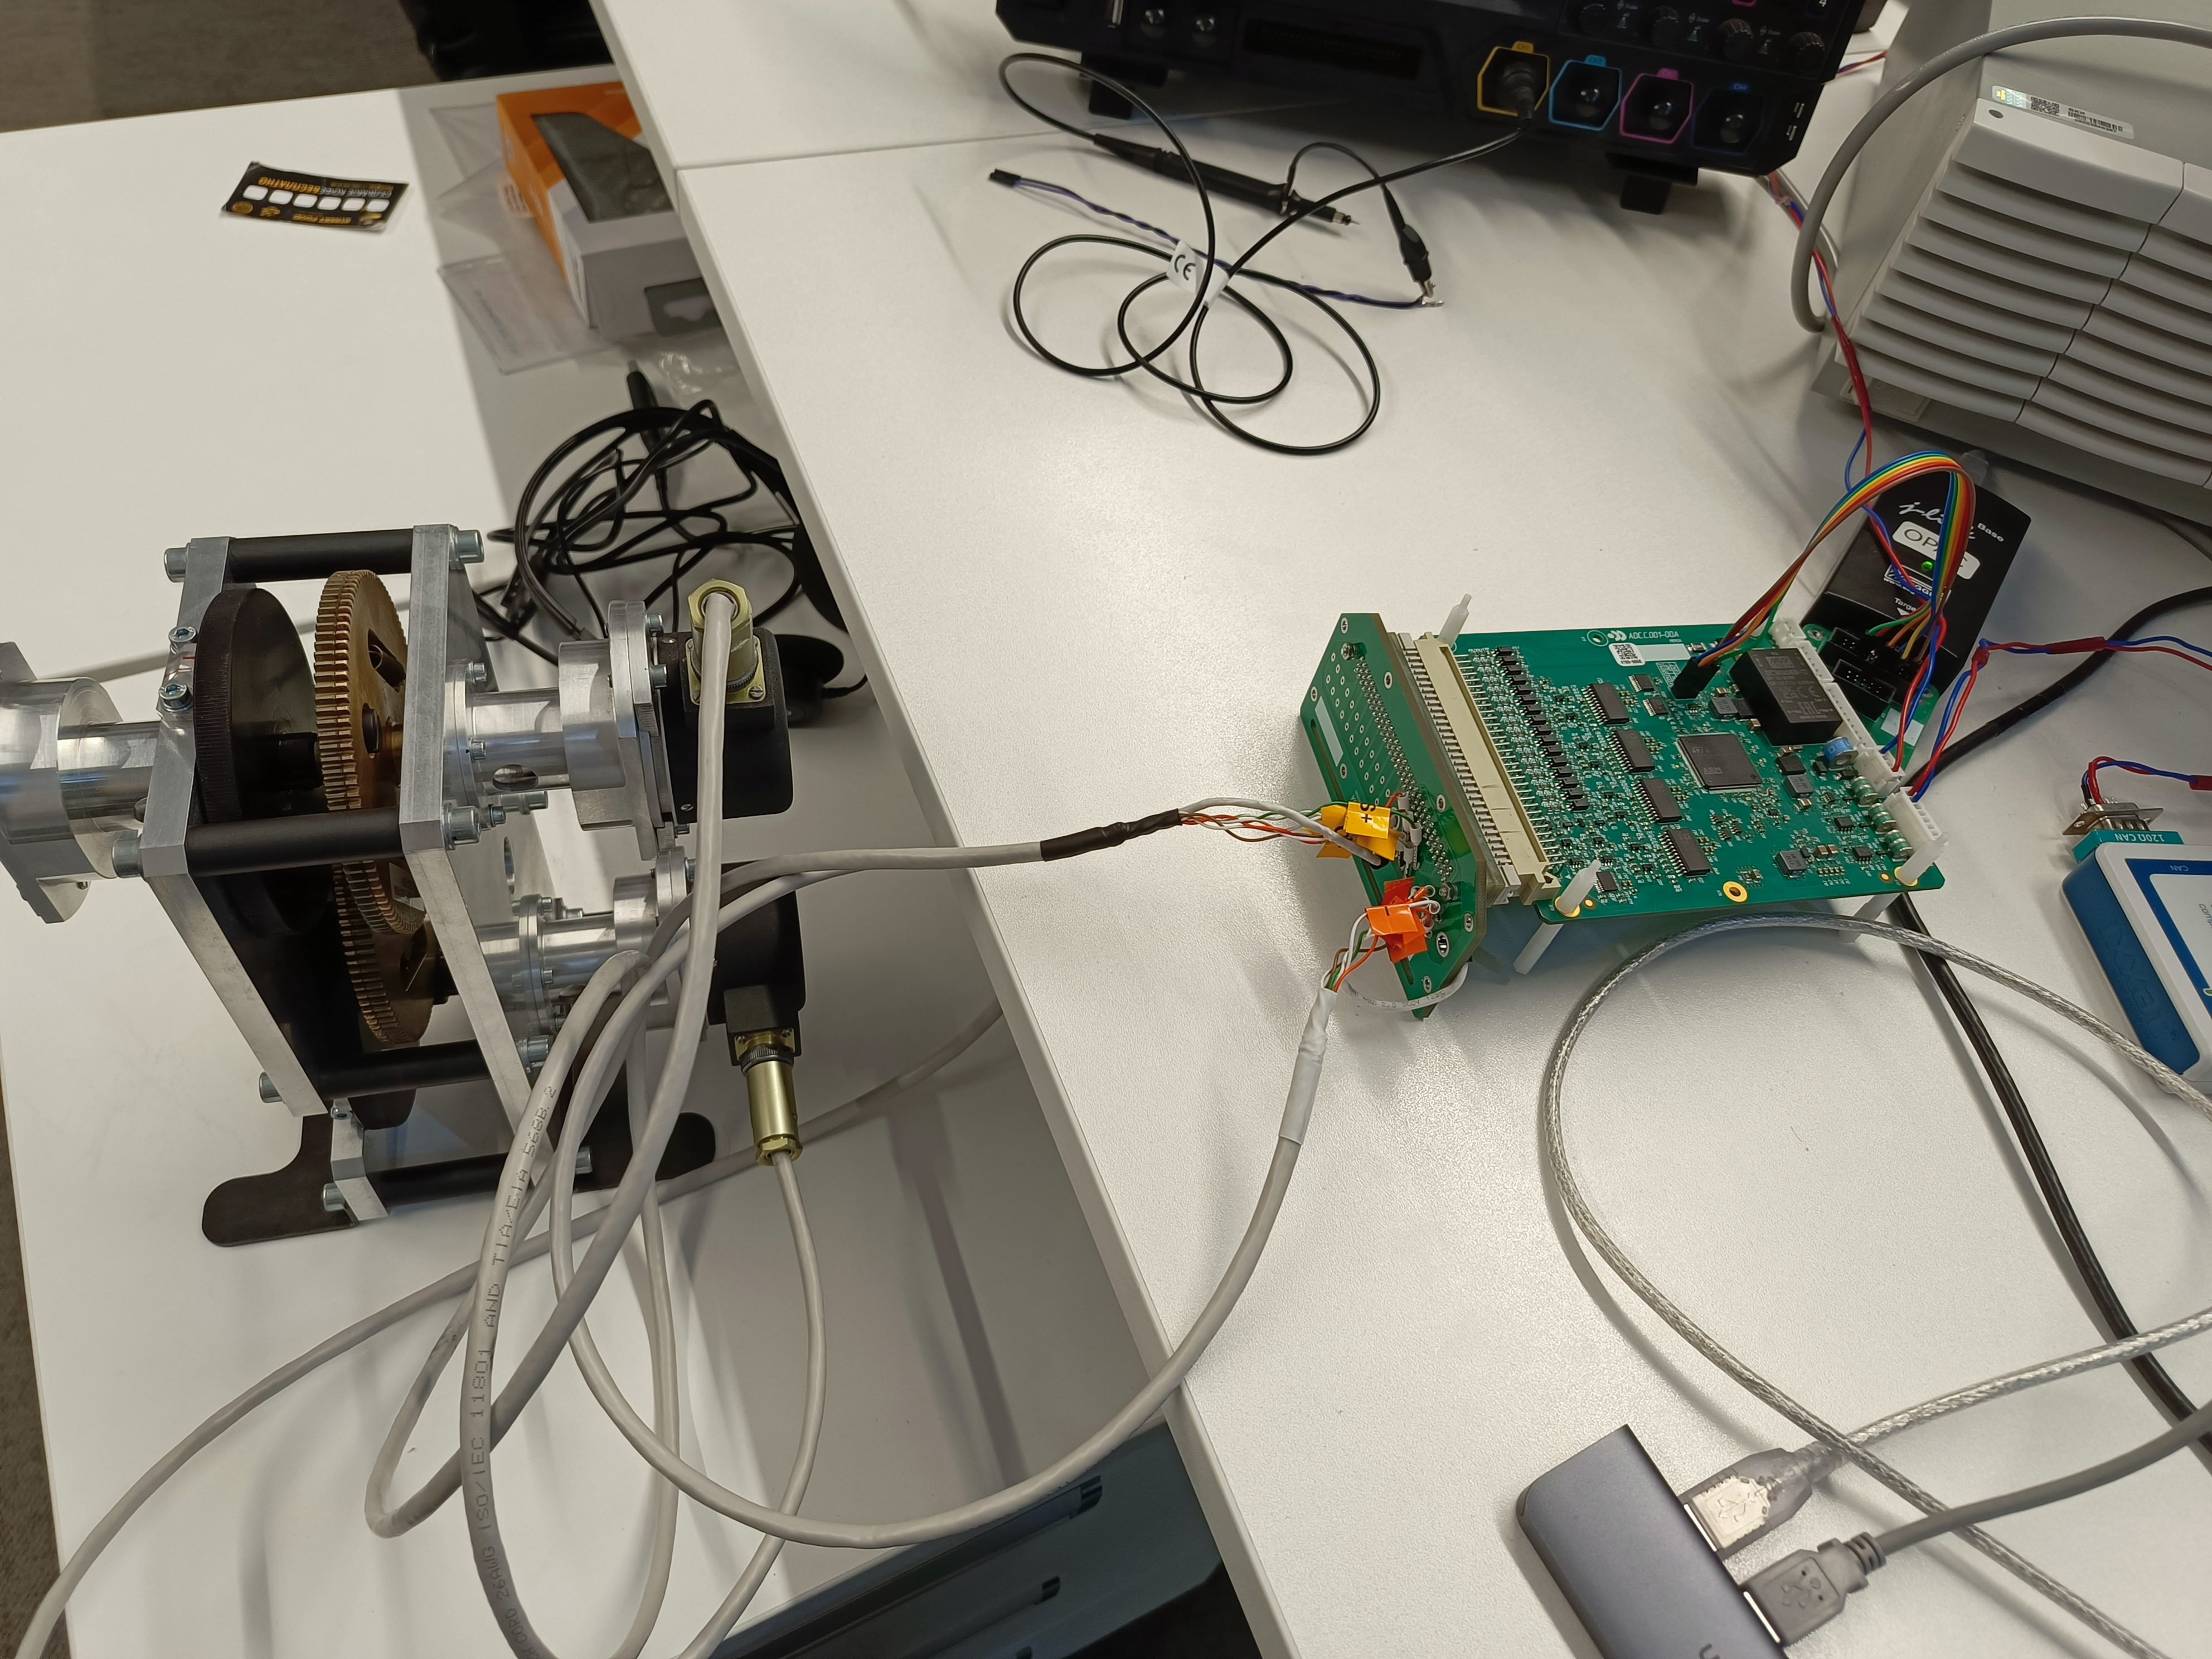
\includegraphics[width=\linewidth]{STND1.jpg} 
    \label{STND1}
  \end{subfigure}
  \hfill
  \begin{subfigure}[b]{0.35\textwidth}
    \centering
    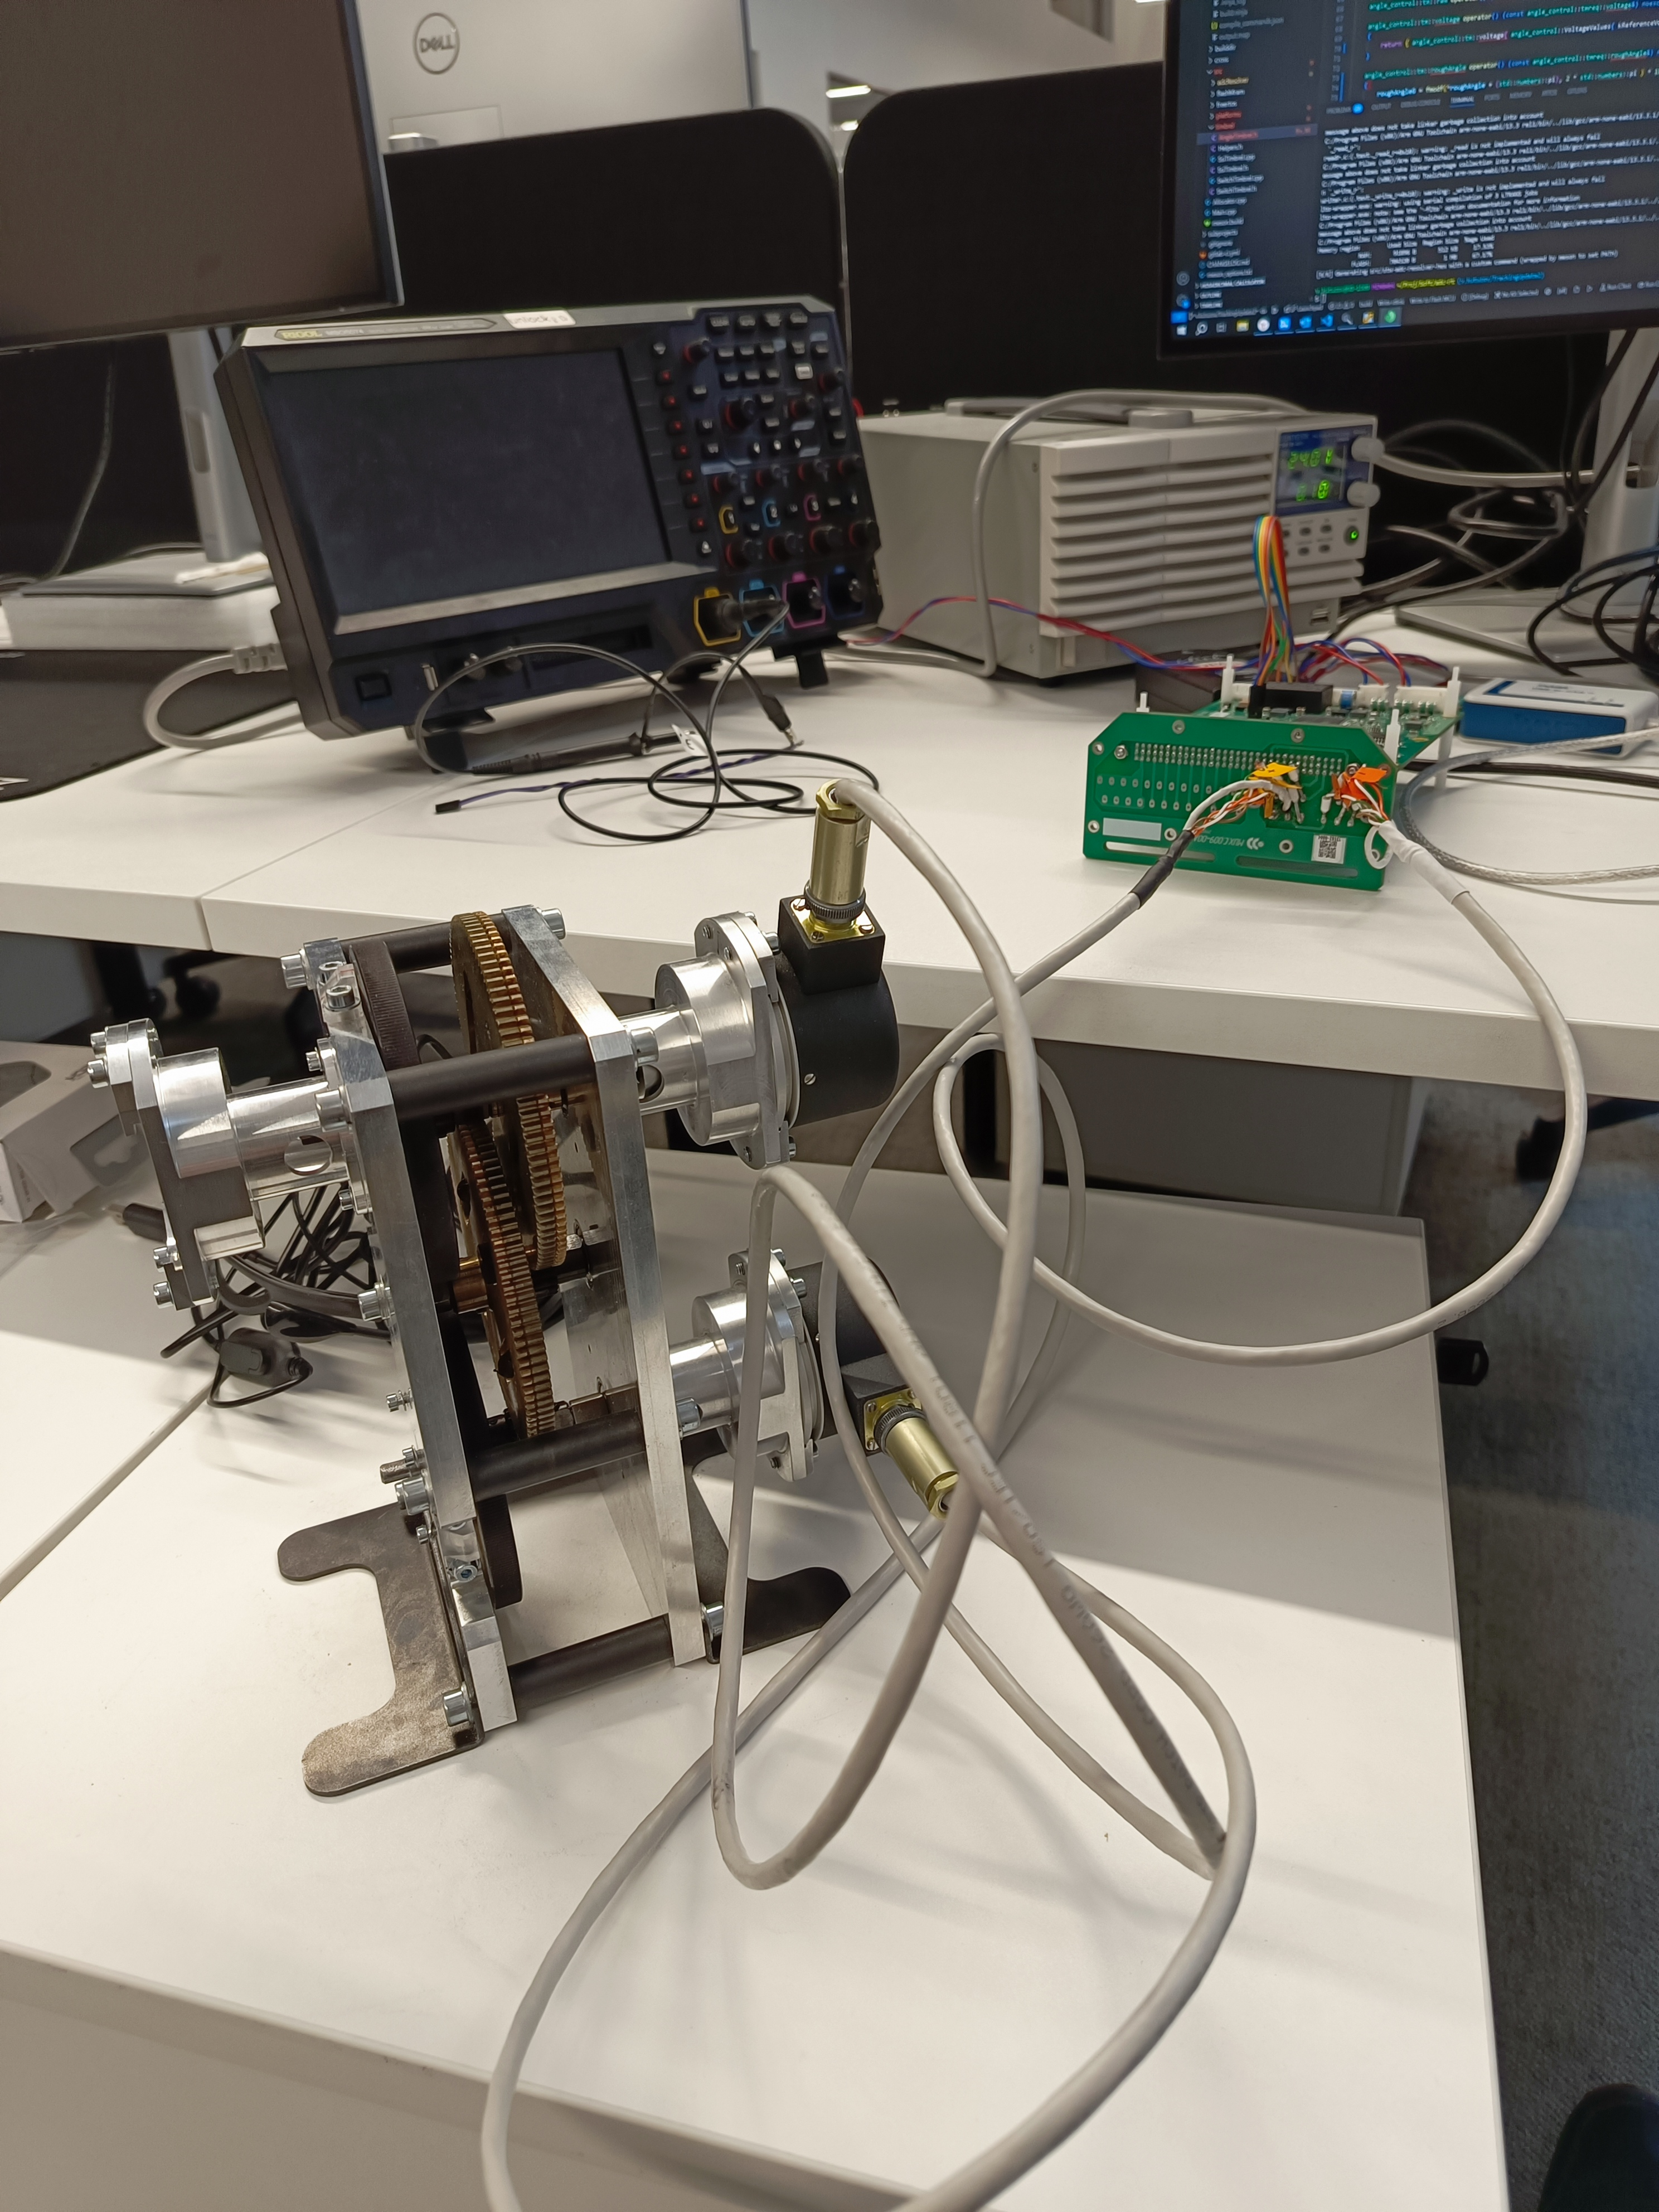
\includegraphics[width=\linewidth]{STND2.jpg} 
    \label{STND2}
  \end{subfigure}

  \caption{Стенд отладки следящего алгоритма}
  \label{STND} 
\end{figure}

Сигналы поступающие в датчик из схемы ЦАП с усилением \textbf{картинка синуса в датчик}
Сигналы с датчика поступающие на АЦП \textbf{картинка кинсуов с датчика}